\documentclass{article}

\usepackage[utf8]{inputenc}
\usepackage[T1]{fontenc}
\usepackage{lipsum}
\usepackage{graphicx}
\usepackage{amsmath}
\usepackage[margin=1in]{geometry}
\usepackage{titlesec}
\usepackage{parskip}
\usepackage{tcolorbox}

\titleformat{\section}
{\LARGE\bfseries}{\thesection}{1em}{}

\titleformat{\subsection}
{\Large\bfseries}{\thesection}{1em}{}

\begin{document}

\pagestyle{empty}

\section*{Type classes}
\large

Haskell appartiene ad una famiglia di linguaggi funzionali fortemente tipati, dove però il programmatore non è forzato a specificare il tipo in maniera esplicita. Sarà il compilatore che andrà ad inferire il tipo in base all'utilizzo dell'entità. Si parla di \textbf{type inference}, anche se sarebbe più corretto parlare in questo caso di \textbf{type reconstruction}.

Volendo dare una definizione più precisa, si suddividono in:
\begin{itemize}
    \item \textbf{Type checking}: il processo attraverso cui il compilatore verifica che un programma sia \textit{tipicamente corretto}, ovvero che ogni espressione sia usata coerentemente con il tipo previsto. Questo può avvenire sia in presenza che in assenza di annotazioni esplicite, ed è fondamentale per garantire la sicurezza e l'affidabilità del codice.
    \item \textbf{Type inference}: il processo attraverso cui il compilatore deduce automaticamente il tipo di un'espressione partendo da annotazioni di tipo già presenti nel programma (ad esempio nei parametri di funzione), propagando queste informazioni nel contesto.
    \item \textbf{Type reconstruction}: un caso più generale di type inference, in cui il compilatore è in grado di dedurre \textit{tutti} i tipi anche in assenza completa di annotazioni, ricostruendo l'intera struttura dei tipi sulla base dell'uso delle entità nel codice.
\end{itemize}

In sintesi, \textbf{type checking}, \textbf{type inference} e \textbf{type reconstruction} sono concetti strettamente correlati nell'ambito dei linguaggi fortemente tipati.\\
Il \textbf{type checking} verifica che i tipi siano usati in modo corretto all'interno del programma.\\
La \textbf{type inference} entra in gioco quando parte delle informazioni di tipo sono disponibili (ad esempio tramite annotazioni) e il compilatore completa le parti mancanti.\\
La \textbf{type reconstruction} è una forma più potente di inferenza, dove il compilatore è in grado di ricostruire interamente i tipi anche in assenza totale di annotazioni. 

In linguaggi come Haskell, la type reconstruction è una caratteristica fondamentale e consente di scrivere codice estremamente conciso mantenendo al contempo un alto livello di sicurezza tipologica.

Ovviamente il programma deve essere scritto correttamente, altrimenti il compilatore non sarà capace di inferire alcun tipo (peggio ancora, un tipo diverso da quello desiderato).

Questo avviene anche in altri linguaggi convenzionali, come in Java e C++, ma vengono considerate eccezzioni. In linguaggi come Haskell questa caratteristica è innata.

Un possibile esempio di type inference in linguaggio Standard ML può essere:
\begin{tcolorbox}
\begin{verbatim}
val a = 3 * 3
val b = 3.14 * 3.14
\end{verbatim}
\end{tcolorbox}
In questo caso sarà il compilatore ad inferire il tipo delle due variabili.\\
Nel caso di \texttt{a} il tipo scelto sarà \texttt{int}, mentre per \texttt{b} sarà \texttt{float}.

\pagebreak

Si osservi ora un esempio di codice rifiutato dal compilatore Standard ML:
\begin{tcolorbox}
\begin{verbatim}
fun square x = x * x
val a = square 3
val b = square 3.14
\end{verbatim}
\end{tcolorbox}
Il compilatore Standard ML restituirà un errore di tipo per una delle due variabili, causato dal fatto che \texttt{square} può restituire due tipi differenti. Se il compilatore scegliesse il tipo \texttt{int} come tipo da restituire, il compilatore restituirebbe un errore per la variabile \texttt{b}.

In OCaml la situazione non è migliore. Riprendendo un esempio simile al precedente:
\begin{tcolorbox}
\begin{verbatim}
let a = 3 * 3
let b = 3.14 *. 3.14
\end{verbatim}
\end{tcolorbox}
Per evitare questo tipo di problemi, in OCaml viene utilizzato un nuovo operatore aritmetico nel caso delle operazioni con floating point (\texttt{*.}).
\begin{tcolorbox}
\begin{verbatim}
let squareI x = x * x
let squareF x = x *. x
let a = squareI 3
let b = squareF 3.14
\end{verbatim}
\end{tcolorbox}
Questo approccio non è scalabile, volendo introdurre altri tipi numerici si dovrebbe creare un nuovo operatore aritmetico ogni volta.\vspace{8pt}\\
Un altro caso spinoso è quello dell'uguaglianza. Si osservi un esempio in OCaml:
\begin{tcolorbox}
\begin{verbatim}
let rec member x = function
        [] -> false
    | (y :: ys) -> x == y || member x ys
;;
val member : ’a -> ’a list -> bool = <fun>
\end{verbatim}
\end{tcolorbox}
Usare \texttt{member} su una lista di funzioni (o di altri elementi che non supportano una nozione di uguaglianza) causa un \textbf{errore a run-time}.

Riprendendo lo stesso esempio in Standard ML:
\begin{tcolorbox}
\begin{verbatim}
fun member (x, [])     = false
    member (x, h :: y) = x == h orelse member x ys
;
val member : "a * "a list -> bool = <fun>
\end{verbatim}
\end{tcolorbox}
In questo caso, le variabili di tipo \texttt{"a} possono essere istanziate solo con tipi per i quali è definita una nozione di uguaglianza.

In Standard ML, se una variabile viene preceduta da un singolo apice (\texttt{'}), la variabile potrà essere istanziata con un qualsiasi tipo arbitrario. Se invece è preceduta da un doppio apice (\texttt{"}), la variabile potrà essere istanziata solo con tipi per i quali è definita una nozione di uguaglianza.

Questa soluzione risulta essere migliore rispetto a quella di OCaml ma resta incompleta, non comprendendo altre proprietà possibili dei tipi.\vspace{14pt}\\
Haskell cerca di risolvere questi problemi cercando di introdurre meccanismi più generici, e non ad hoc come quelli discussi precedentemente.

In Haskell, i tipi sono divisi in \textbf{classi}, non necessariamente disgiunte. Ogni classe è definita dalle \textbf{operazioni} supportate da quei tipi. Alcuni esempi possono essere:
\begin{tcolorbox}
\begin{verbatim}
(+)     :: Num a            => a -> a -> a
negate  :: Num a            => a -> a
recip   :: Fractional a     => a -> a
sin     :: Floating a       => a -> a
(==)    :: Eq a             => a -> a -> Bool
(<=)    :: Ord a            => a -> a -> Bool
min     :: Ord a            => a -> a -> a
\end{verbatim}
\end{tcolorbox}

Di seguito alcune delle classi principali presenti, rappresentate attraverso un diagramma dove le classi sono di colore \textit{rosso} ed i tipi di colore \textit{blu}:
\begin{center}
    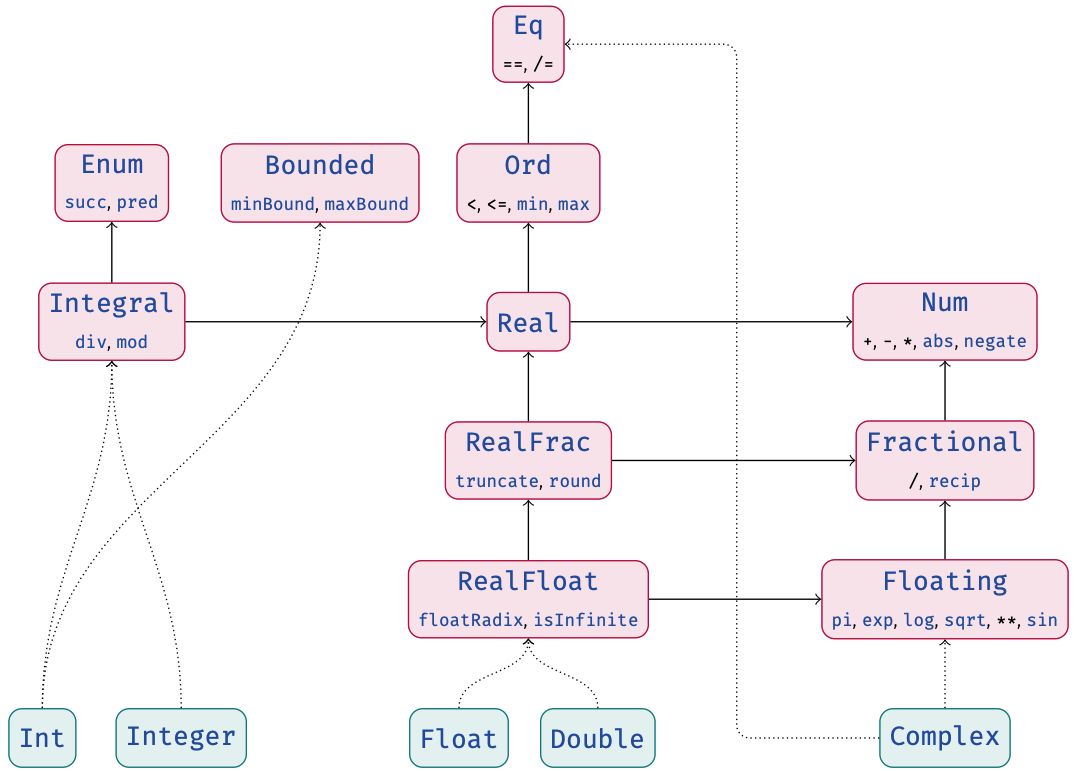
\includegraphics[width=\textwidth]{img/classes.png}
\end{center}

Per definire una nuova classe di tipi in Haskell la sintassi da utilizzare è la seguente:
\begin{tcolorbox}
\begin{verbatim}
class Num a where
    (+), (-), (*)   :: a -> a -> a
    negate, abs     :: a -> a
\end{verbatim}
\end{tcolorbox}
All'interno della classe vengono definite le funzioni che la variabile \texttt{a} di classe \texttt{Num} deve possedere.

Per ogni tipo \texttt{a} della classe \texttt{Num} sono definite le operazioni \texttt{(+), (-), ...} il cui significato (implementazione) dipende dal tipo effettivo con cui viene istanziata \texttt{a}.

Due esempi possono essere:
\begin{tcolorbox}
\begin{verbatim}
square :: Num a => a -> a
square = x * x

member :: Eq a => a -> [a] -> Bool
member _ []         = False
member x (y : ys)   = x == y || member x ys
\end{verbatim}
\end{tcolorbox}
\vspace{8pt}
Una volta definita una classe di tipo la si può popolare (un tipo appartiene a questa classe) definendo una nuova istanza di quella classe.

Per definire una nuova istanza di una classe in Haskell la sintassi da utilizzare è la seguente:
\begin{tcolorbox}
\begin{verbatim}
instance Num Int where
    (+)     = addInt
    (-)     = subInt
    (*)     = mulInt
    negate  = negateInt
    abs     = absInt

instance Num Float where
    (+)     = addFloat
    (-)     = subFloat
    (*)     = mulFloat
    negate  = negateFloat
    abs     = absFloat
\end{verbatim}
\end{tcolorbox}

Per ogni tipo, si dovranno definire le realizzazioni concrete delle funzioni presenti nella classe.

In questo caso, \texttt{addInt, mulFloat, ...} sono le funzioni primitive per sommare numeri interi, moltiplicare numeri floating-point, ecc.

Non ci sono vincoli su dove definire o istanziare le classi, a differenza dei trait in Go.

\pagebreak

Due classi molto importanti in Haskell sono le classi \textbf{Show} e \textbf{Read}.
\begin{tcolorbox}
\begin{verbatim}
show :: Show a => a -> String

read :: Read a => String -> a
\end{verbatim}
\end{tcolorbox}
\texttt{show} è la funzione analoga al metodo \texttt{toString()} in Java. Crea la rappresentazione testuale di un dato. Non è quindi possibile rappresentare in stringa qualsiasi tipo di dato, come ad esempio le funzioni.

\texttt{read} è la funzione inversa di \texttt{show}. E' in grado di costruire un valore di tipo arbitrario a partire da una stringa. Anche in questo caso, non è sempre possibile rappresentare un tipo di dato partendo da una stringa.

\texttt{show} è una funzione \textbf{totale} (per ogni valore di tipo \texttt{a} della classe \texttt{show} viene prodotta una stringa), al contrario \texttt{read} è necessariamente \textbf{parziale} (non sempre si può effettuare un parsing di un tipo da una stringa).\vspace{14pt}\\
In Haskell, anche le costanti sono polimorfe. Un esempio sulle costanti numeriche può essere:
\begin{tcolorbox}
\begin{verbatim}
ghci> :t 42
42 :: Num a => a

ghci> :t 42.5
42.5 :: Fractional a => a

ghci> :t pi
pi :: Floating a => a
\end{verbatim}
\end{tcolorbox}
Haskell riesce a rimanere su un tipo vago (classe \texttt{Num}) finché non viene aggiunto un livello di dettaglio maggiore. Anche nel secondo esempio, si rimane vaghi con la classe \texttt{Fractional}.\vspace{14pt}\\
E' possibile inoltre definire sottoclassi. Un possibile esempio può essere:
\begin{tcolorbox}
\begin{verbatim}
class Eq a => Ord a where
    compare :: a -> a -> Ordering
    (<)     :: a -> a -> Bool
    (<=)    :: a -> a -> Bool
    (>)     :: a -> a -> Bool
    (>=)    :: a -> a -> Bool
    max     :: a -> a -> a
    min     :: a -> a -> a
\end{verbatim}
\end{tcolorbox}
In questo caso, la classe \texttt{Ord} è sottoclasse di \texttt{Eq}.

\pagebreak

E' possibile anche fornire delle implementazioni di default. Un possibile esempio può essere:
\begin{tcolorbox}
\begin{verbatim}
class Eq a where
    (==) :: a -> a -> Bool
    (/=) :: a -> a -> Bool

    x == y = not (x /= y)       // implementazione di default
    x /= y = not (x == y)       // implementazione di default
\end{verbatim}
\end{tcolorbox}
Basta implementare una delle due operazioni per avere automaticamente l’implementazione dell’altra.\vspace{14pt}\\
Si possono definire anche istanze generiche. Un possibile esempio può essere:
\begin{tcolorbox}
\begin{verbatim}
instance Eq a => Eq [a] where
    [] == []                = True
    (x :: xs) == (y :: ys)  = x == y && xs == ys
    _ == _                  = False
\end{verbatim}
\end{tcolorbox}
In questo caso, per definire una nozione di uguaglianza tra liste è necessario (e sufficiente) che esista una nozione di uguaglianza tra gli elementi di tali liste.

La nozione di disuguaglianza è definita \textit{implicitamente} come negazione dell’uguaglianza.\vspace{14pt}\\
Dopo l'introduzione delle classi di tipo, ci si è resi conto che poteva essere utile introdurre anche delle classi su costruttori di tipo.

Per \textbf{costruttore di tipo} si intende una funzione che applicata ad un tipo produce un tipo.

Ad esempio, una lista da sola non rappresenta un tipo, ma un costruttore di tipo.\\
Una lista associata ad un tipo è un tipo, come una lista di interi.

Un ulteriore esempio di costruttore di tipo in Haskell è \texttt{Maybe} (simile all'Optional in Java).\\
\texttt{Maybe} si divide in \texttt{Just valore} e \texttt{Nothing}. Si può associare al costruttore \texttt{Maybe} un tipo.

Ad esempio, all'interno della libreria standard di Haskell è presente il seguente codice:
\begin{tcolorbox}
\begin{verbatim}
class Foldable t where
    length  :: t a -> Int
    sum     :: Num a => t a -> a

class Functor t where
    fmap    :: (a -> b) -> t a -> t b
\end{verbatim}
\end{tcolorbox}
Le \texttt{t} in questo codice indicano costruttori di tipo. Associando \texttt{t} ad \texttt{a} viene creato un tipo.

\texttt{Foldable} viene utilizzato per rappresentare strutture dati (contenitori) che possono essere “ridotte” a un singolo valore. Su dei contenitori ha senso avere come operazioni il calcolo della lunghezza del contenitore e della somma degli elementi presenti nel contenitore (sono presenti anche altre operazioni, come \texttt{product} e \texttt{null}).

\texttt{Functor} viene utilizzato per rappresentare contenitori su cui puoi applicare una funzione a ogni elemento senza cambiare la struttura del contenitore.\\
\texttt{fmap} prende una funzione da \texttt{a} a \texttt{b} e la applica a ogni \texttt{a} all'interno del contenitore \texttt{f a}, restituendo \texttt{f b}.\\
Un possibile esempio di utilizzo può essere \texttt{fmap (+1) [1,2,3]}, con risultato \texttt{[2,3,4]}.



\end{document}